\documentclass[12pt]{article}  % [12pt] option for the benefit of aging markers
\usepackage{amssymb,amsthm}    % amssymb package contains more mathematical symbols
\usepackage{graphicx}          % graphicx package enables you to paste in graphics
\usepackage[document]{ragged2e} 
\usepackage{float}
\usepackage{tabularx}
\usepackage{multirow}

%%%%%%%%%%%%%%%%%%%%%%%%%%%%%%%%%
%
%    Page size commands.  Don't worry about these
%
\setlength{\textheight}{220mm}
\setlength{\topmargin}{-10mm}
\setlength{\textwidth}{150mm}
\setlength{\oddsidemargin}{0mm}

%%%%%%%%%%%%%%%%%%%%%%%%%%%%%%%%%%%%%%%%%%%%%%%%%%%%%%%%%%%%%%%
%
%    Definitions of environments for theorems etc.
%
\newtheorem{theorem}{Theorem}[section]          % Theorems numbered within sections - eg Theorem 2.1 in Section 2.
\newtheorem{corollary}[theorem]{Corollary}      % Corollaries etc. will be counted as Theorems for numbering
\newtheorem{lemma}[theorem]{Lemma}              % eg Lemma 3.1, ... Theorem 3.2, ... Corollary 3.3.
\newtheorem{proposition}[theorem]{Proposition}
\newtheorem{conjecture}[theorem]{Conjecture}

\theoremstyle{definition}
\newtheorem{definition}[theorem]{Definition}

\theoremstyle{remark}
\newtheorem{remark}[theorem]{Remark}
\newtheorem{example}[theorem]{Example} 
\graphicspath{ {./Images/} }

%%%%%%%%%%%%%%%%%%%%%%%%%%%%%%%%%%%%%%%%%%%%%%%
%
%        Preamble material specific to your essay
%
\title{Evaluation of Mastermind Solutions\\
Deliverable 1: Research Report}
\author{Kyle Dick\\
F20PA Project\\
supervised by
Kathrin Stark}

\begin{document}
\maketitle

\newpage                     % optional page break
\begin{abstract}
Describe the problem that is to be approached.


\end{abstract}

\newpage                     % optional page break
\tableofcontents

\newpage                     % optional page break
\section{Introduction}\label{s:intro}
%
%In recent times a global interest has developed around the linguistic game Wordle. The concept of this puzzle is simple, the user is to guess a five letter word in as few guesses as possible within six attempts. After each guess the computer will inform the user if a letter was in the correct position, denoted as a green highlight, or is contained within the word but not in the correct %position, denoted with a yellow highlight.
The main focus of this project is to investigate solutions to the puzzle game known as Mastermind. The approach will be to develop an initial base solution in a functional programming language which can be iteratively improved with the goal of creating a solution which is logically sound and efficient.
Mastermind is a simple code-breaking game in which one player will create a secret code which consists of four coloured pegs from a choice of six. This is the standard version of the game however there are multiple variations of the game, some of which will be discussed and examined within the scope of this project.

\subsection {Aims and Objectives}
The aims and objectives of this project can be surmised in two specific goals. The first goal is to derive a solution to the logical puzzle Mastermind. The second goal is to evaluate solutions implemented during this project with the aim to find methods to improve later iterations. An in depth explanation of the chosen aims and objectives are as such:

\

\textbullet\ Aim 1: To derive a solution to the puzzle Mastermind.

\

 The goal to find a solution to the problem which minimizes the number of guesses required to discover the correct combination of pegs which comprise the code. Intially the goal will be to derive a base solution to the Mastermind puzzle. The base solution being the most intuitive solution to the problem which does not aim to be the most efficient but to provide a foundation on which improvements can be made. The following objectives are associated with this aim:

\

\textbullet\ Objective 1.A: Investigate the problem space.

\

The Mastermind puzzle has previously been the subject of similar research regarding the ability to efficiently find the correct code combination. This stage of the project will concern itself with investigating these previous implementations to guide the project. Through exploring the methods utilised in other investigations into this problem the areas in which these solutions are lacking or could be improved can be found. The research presented in this report represents the progress of this objective.

\

\textbullet\ Objective 1.B:  Implement a base solution.

\

The ideal base solution should acheive the basic goal of arriving at the correct code combination but should not be the most elegant solution at this point. Instead the base solution should be the foundation for which improvements are made in later iterations. The base solution will be guided through the research conducted through objective 1.A.

\

\textbullet\ Aim 2: Optimise the Mastermind Solution.

\

The next step following the creation of a base solution is the optimization of this implementation. The goal with optimization is to discover new methods of how the solution can be improved in regards to its efficiency. In the context of the Mastermind puzzle the concept of a search space is an important factor to optimization as it refers to the set of possible codes which satisfy the problem. An example of how the solution could be optimized is by considering ways in which this search space could be either minimized or how the navigation of the space can be improved.

\

\textbullet\ Objective 2.A: Explore Methods of Optimizing the Search Space.

\

The optimization of the problem's search space is directly linked to the measure of efficiency when considering Mastermind solutions. An of how this can be achieved is by implementing methods of minimizing the search space such that the quantity of possible codes which could satisfy the problem is reduced. The other method that should be investigated is improvements to how the search space is navigated by the solution. This is a method which relates heavily to the concept of heuristics and assigning values to the items within the search space which will be covered in a later section of this report. These are not the only methods that exist to optimize the search space and the exploration of differing methods is to be encouraged and sought out should it be possible.

\

\textbullet\ Objective 2.B: Explore Methods of Measuring the Efficiency of a Solution.

\

To achieve the goal of optimizing the solution it is important to define the elements which are being optimized for. An example of this is already defined by the previous objective in regards to search space however this is not the only area which can be optimized. The question that is to be answered by this objective is how other factors such as the speed at which a solution can reach a code which satisfies the problem should be considered.

\

\textbullet\ Objective 2.C: Improve the Solution.

\

This is a continual objective which encapsulates the main goal of this aim. Measurements of the optimization as defined by previous objectives should reflect the improvements made in later iterations of the solution. Documentation of the results of each optimization method should be presented as a component of this objective.

\

\textbullet\ Aim 3: Evaluate Solution.

\

This aim constitutes the final stages of the project. During this stage a final solution should be implementation with appropriate reasoning as to the optimizations which will be compared to already existing solutions. The comparison process should provide insight into the areas which could still be optimized.

\

\textbullet\ Objective 3.A: Design an Evaluation Process.

\

The evaluation process should consider the optimization methods implemented during the development of each solution iteration. It is important that the evaluation process considers factors in which the solution can be compared to similar solutions as to provide reasoning for why one solution may be an improvement over another
This objective is covered in the Evaluation Strategy chapter later in this report

\

\textbullet\ Objective 3.B: Present the Results of the Evaluation Process.

\

The evaluation process provides insight in how an optimization procedure may have given one solution an advantage over a similar implementation. The results of the process should be communicated clearly such that these insights can be reasoned and explained.

\

\textbullet\ Aim 4: Investigate Solutions to Mastermind Variants.

\

This aim and its associated objectives are intended to be goals which are desired to be included with the results of the project but are not fundamental to the investigation. These objectives should be pursued if the time allows for these areas to be explored. The topic of investigation for this aim is to explore how variations of the Mastermind puzzle can be processed by the solution implemented in this project. Possible optimization methods in respect to these changes should be documented and communicated alongside the challenges encountered.

\

\textbullet\ Objective 4.A: Investigate Solution with Variance in Set Size for Possible Symbols.

\

A topic that is a recurring source of intrigue with similar research into the Mastermind puzzle is the potential for a solution to scale with changes in the way that the code is constructed. One such change relates to the possible set of symbols which the code could contain. This objective should consider methods of how the solution can adapt when the number of possible symbol increases above the standard six.

\

\textbullet\ Objective 4.B: Investigate Solution with Variance in Code Length.

\

An additional scaling factor which is an area of possible investigation is changes in the length of the code. The considerations regarding this objective relate to the ways in how a solution will handle the larger search space and the changes in optimization.

\

\textbullet\ Objective 4.C: Investigate Solutions to Similar Problems.

\

The solution implemented in this project could have applications beyond the intial Mastermind puzzle. This objective is concerned with how the solution can be applied to other similar problems, an example of such a puzzle would be the popular language game Wordle \cite{Wordle}.

%
% The \label command is optional, but useful.  To cross-refer to a section/theorem/equation etc.
% labelled by \label{key}, use \ref{key}.  For example: Equation (\ref{eq:key}) follows from Theorem \ref{th:key}.

\newpage                     % optional page break
\section{Background}\label{ss:back}

% Summary of the background material and introduction to the section
This section will provide background material which aims to give context to the aims and objectives of this project. The project was inspired by a paper exploring sudoku solutions from a series of problems known as functional pearls, the processes used to derive those solutions will be used to guide this project in this current stage. Following this brief introduction is an explanation of the game Mastermind which the solution will be derived from along with references to previous work by others. The previous work examined will focus on the specific area of search spaces in regards to finding the optimal best move at each position in the puzzle. At the conclusion of this section the goal is that the reader has an understanding of the important concepts relating to this project such that the aims and objectives are clear in their feasability and relevancy.

%%% What is the problem?
% What is the goal of Mastermind that our solution will be modelled on?
\subsection {Mastermind}

% A brief history and explanation of the game
Mastermind is a two-player code-breaking game centered around a code-maker (CM) who creates a secret code and a code-breaker (CB) who attempts to discover the code \cite{Wolfram}.The physical board game was designed by an Isreali Postmaster named Mordecai Meirowitz and originally manufactured by Invicta Toys and Games \cite{Invicta}. 

% Explanation of Mastermind puzzle
The standard variant of the game plays as follows:
\begin {itemize}
	\item {The $CM$ will create a secret code of length $L$ unknown to $CB$ from a set of symbols $S$, in the physical game these were represented by plastic pegs. In the standard variant $L=4$ and $S=6$  represents a code of four symbols in length constructed from a set of six possible symbols.}
	\begin{figure}[H]
	\centering
	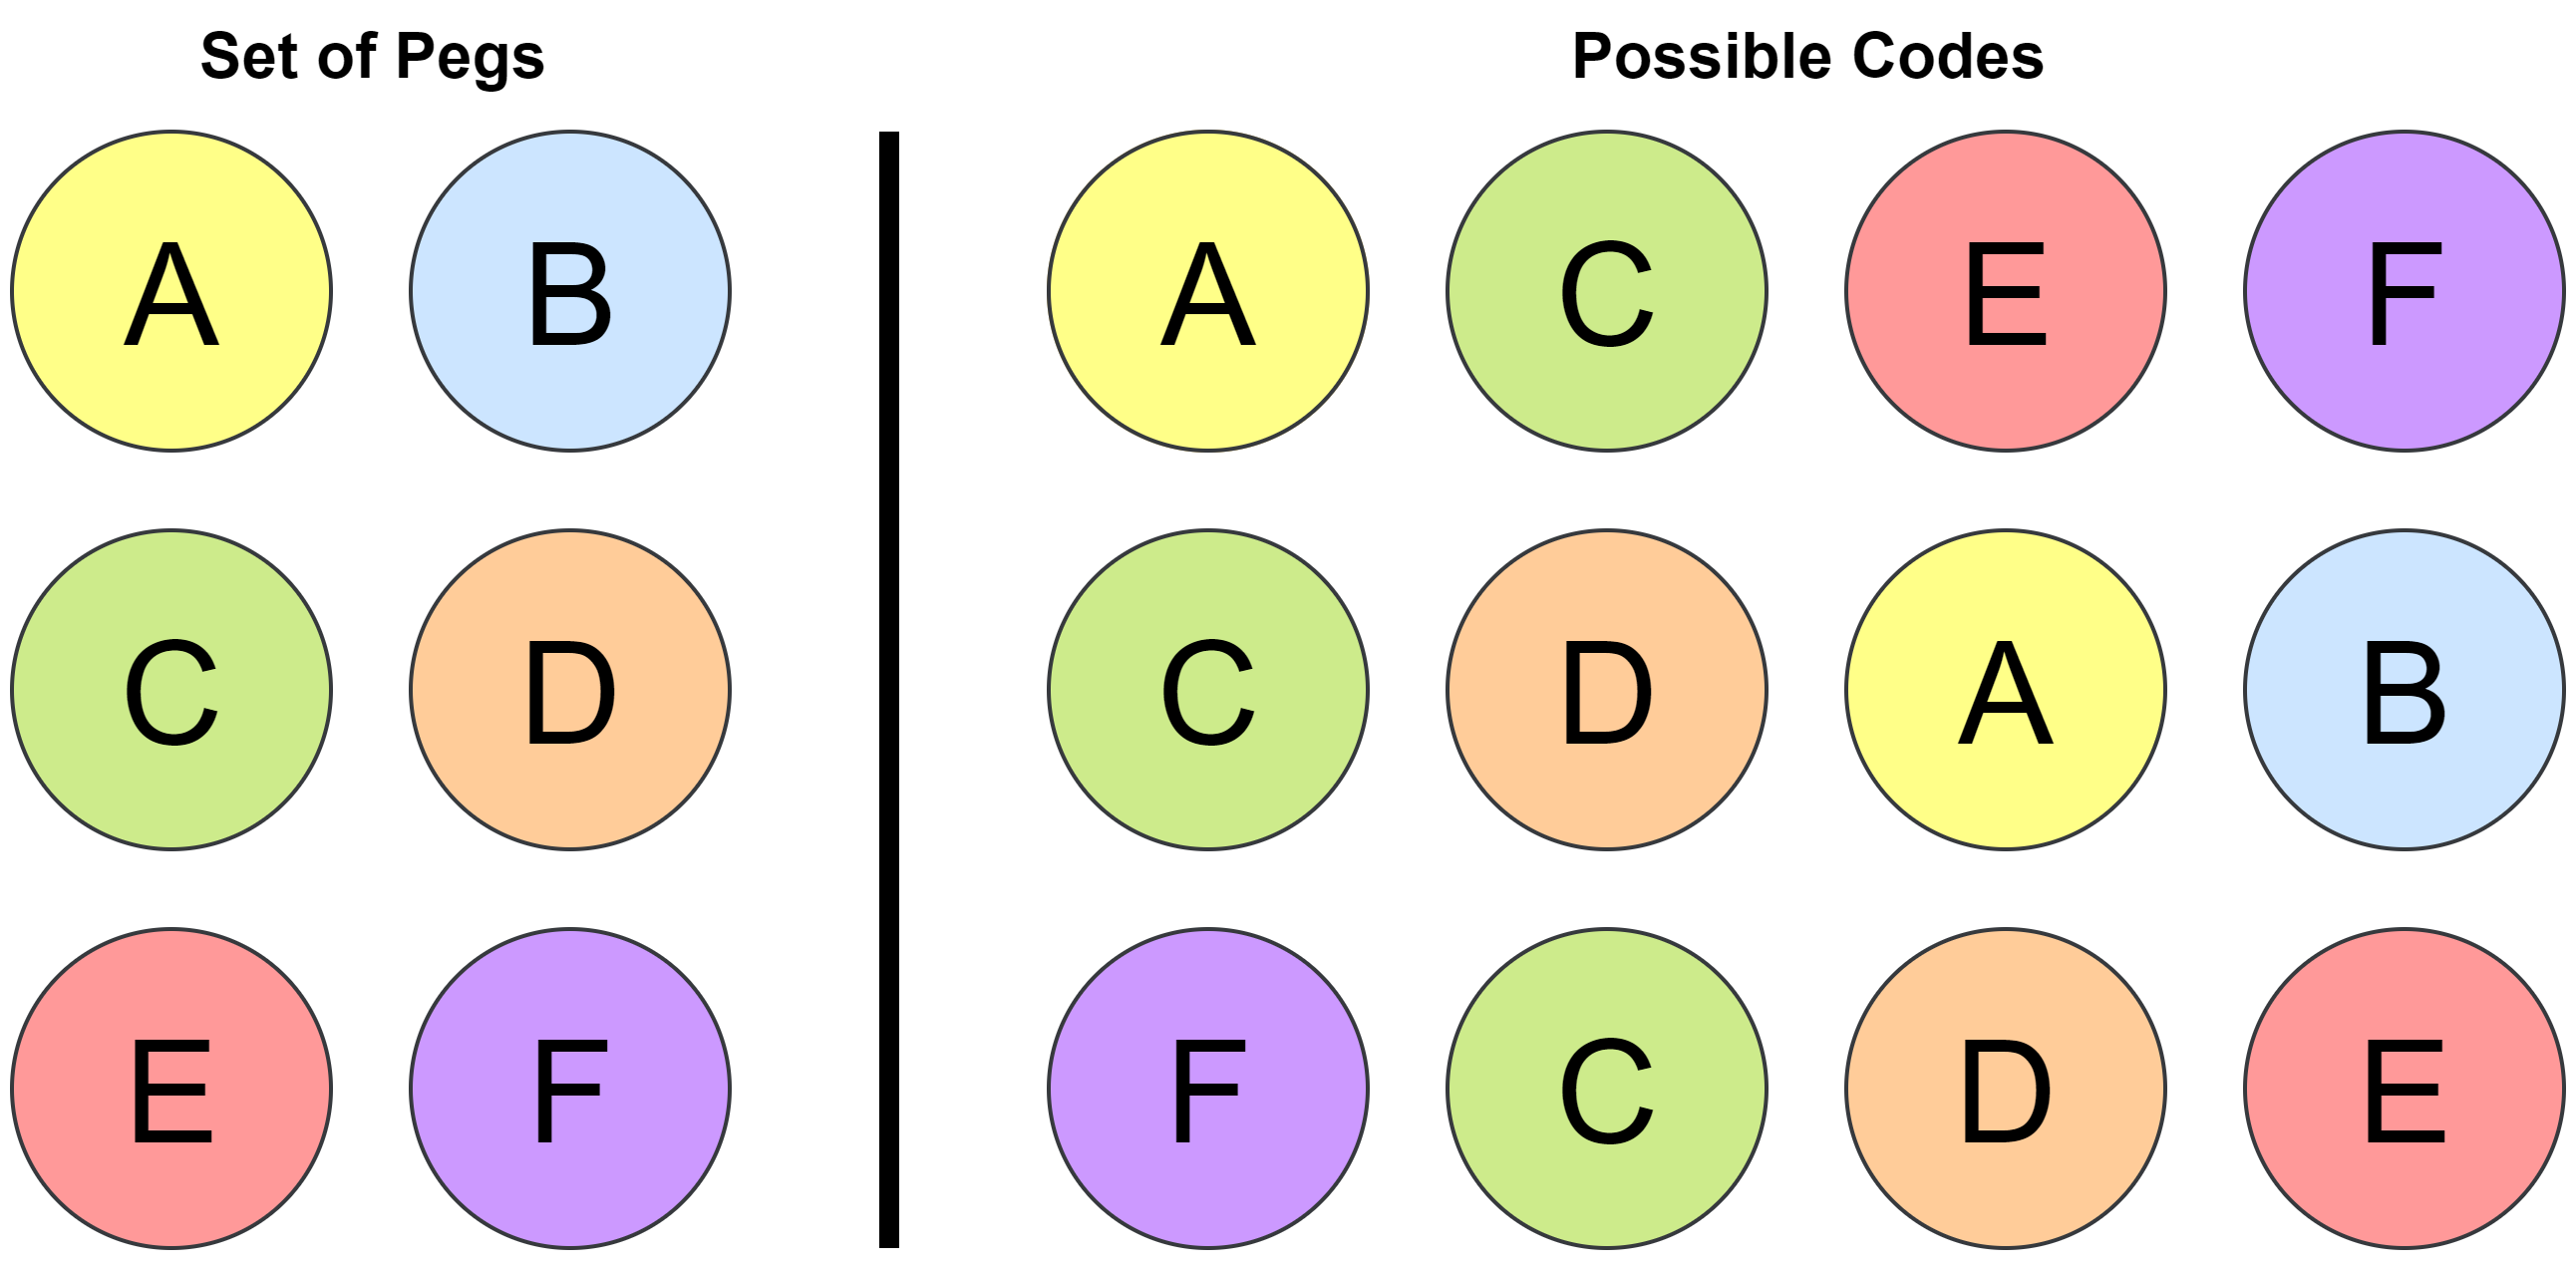
\includegraphics[scale=0.75]{pegs}
	\caption{ Example of code enumerations the $CM$ could construct in the standard variant.}
	\end{figure}
	\item {The $CB$ is tasked with solving the code that the $CM$ has constructed by creating test patterns from $S$. In the physical board game the number of guesses that the $CB$ is allowed is limited to 10 \cite {Nelson}, the size of the plastic board. The test patterns are evaluated by $CM$ through a pair of indicators. The first indicator, represented by a white plastic peg in the physical game, denotes that a correct symbol was used but in an incorrect position. The second indicator, represented by a black plastic peg, denotes that a correct symbol was used in the correct position.}
	\begin{figure}[H]
	\centering
	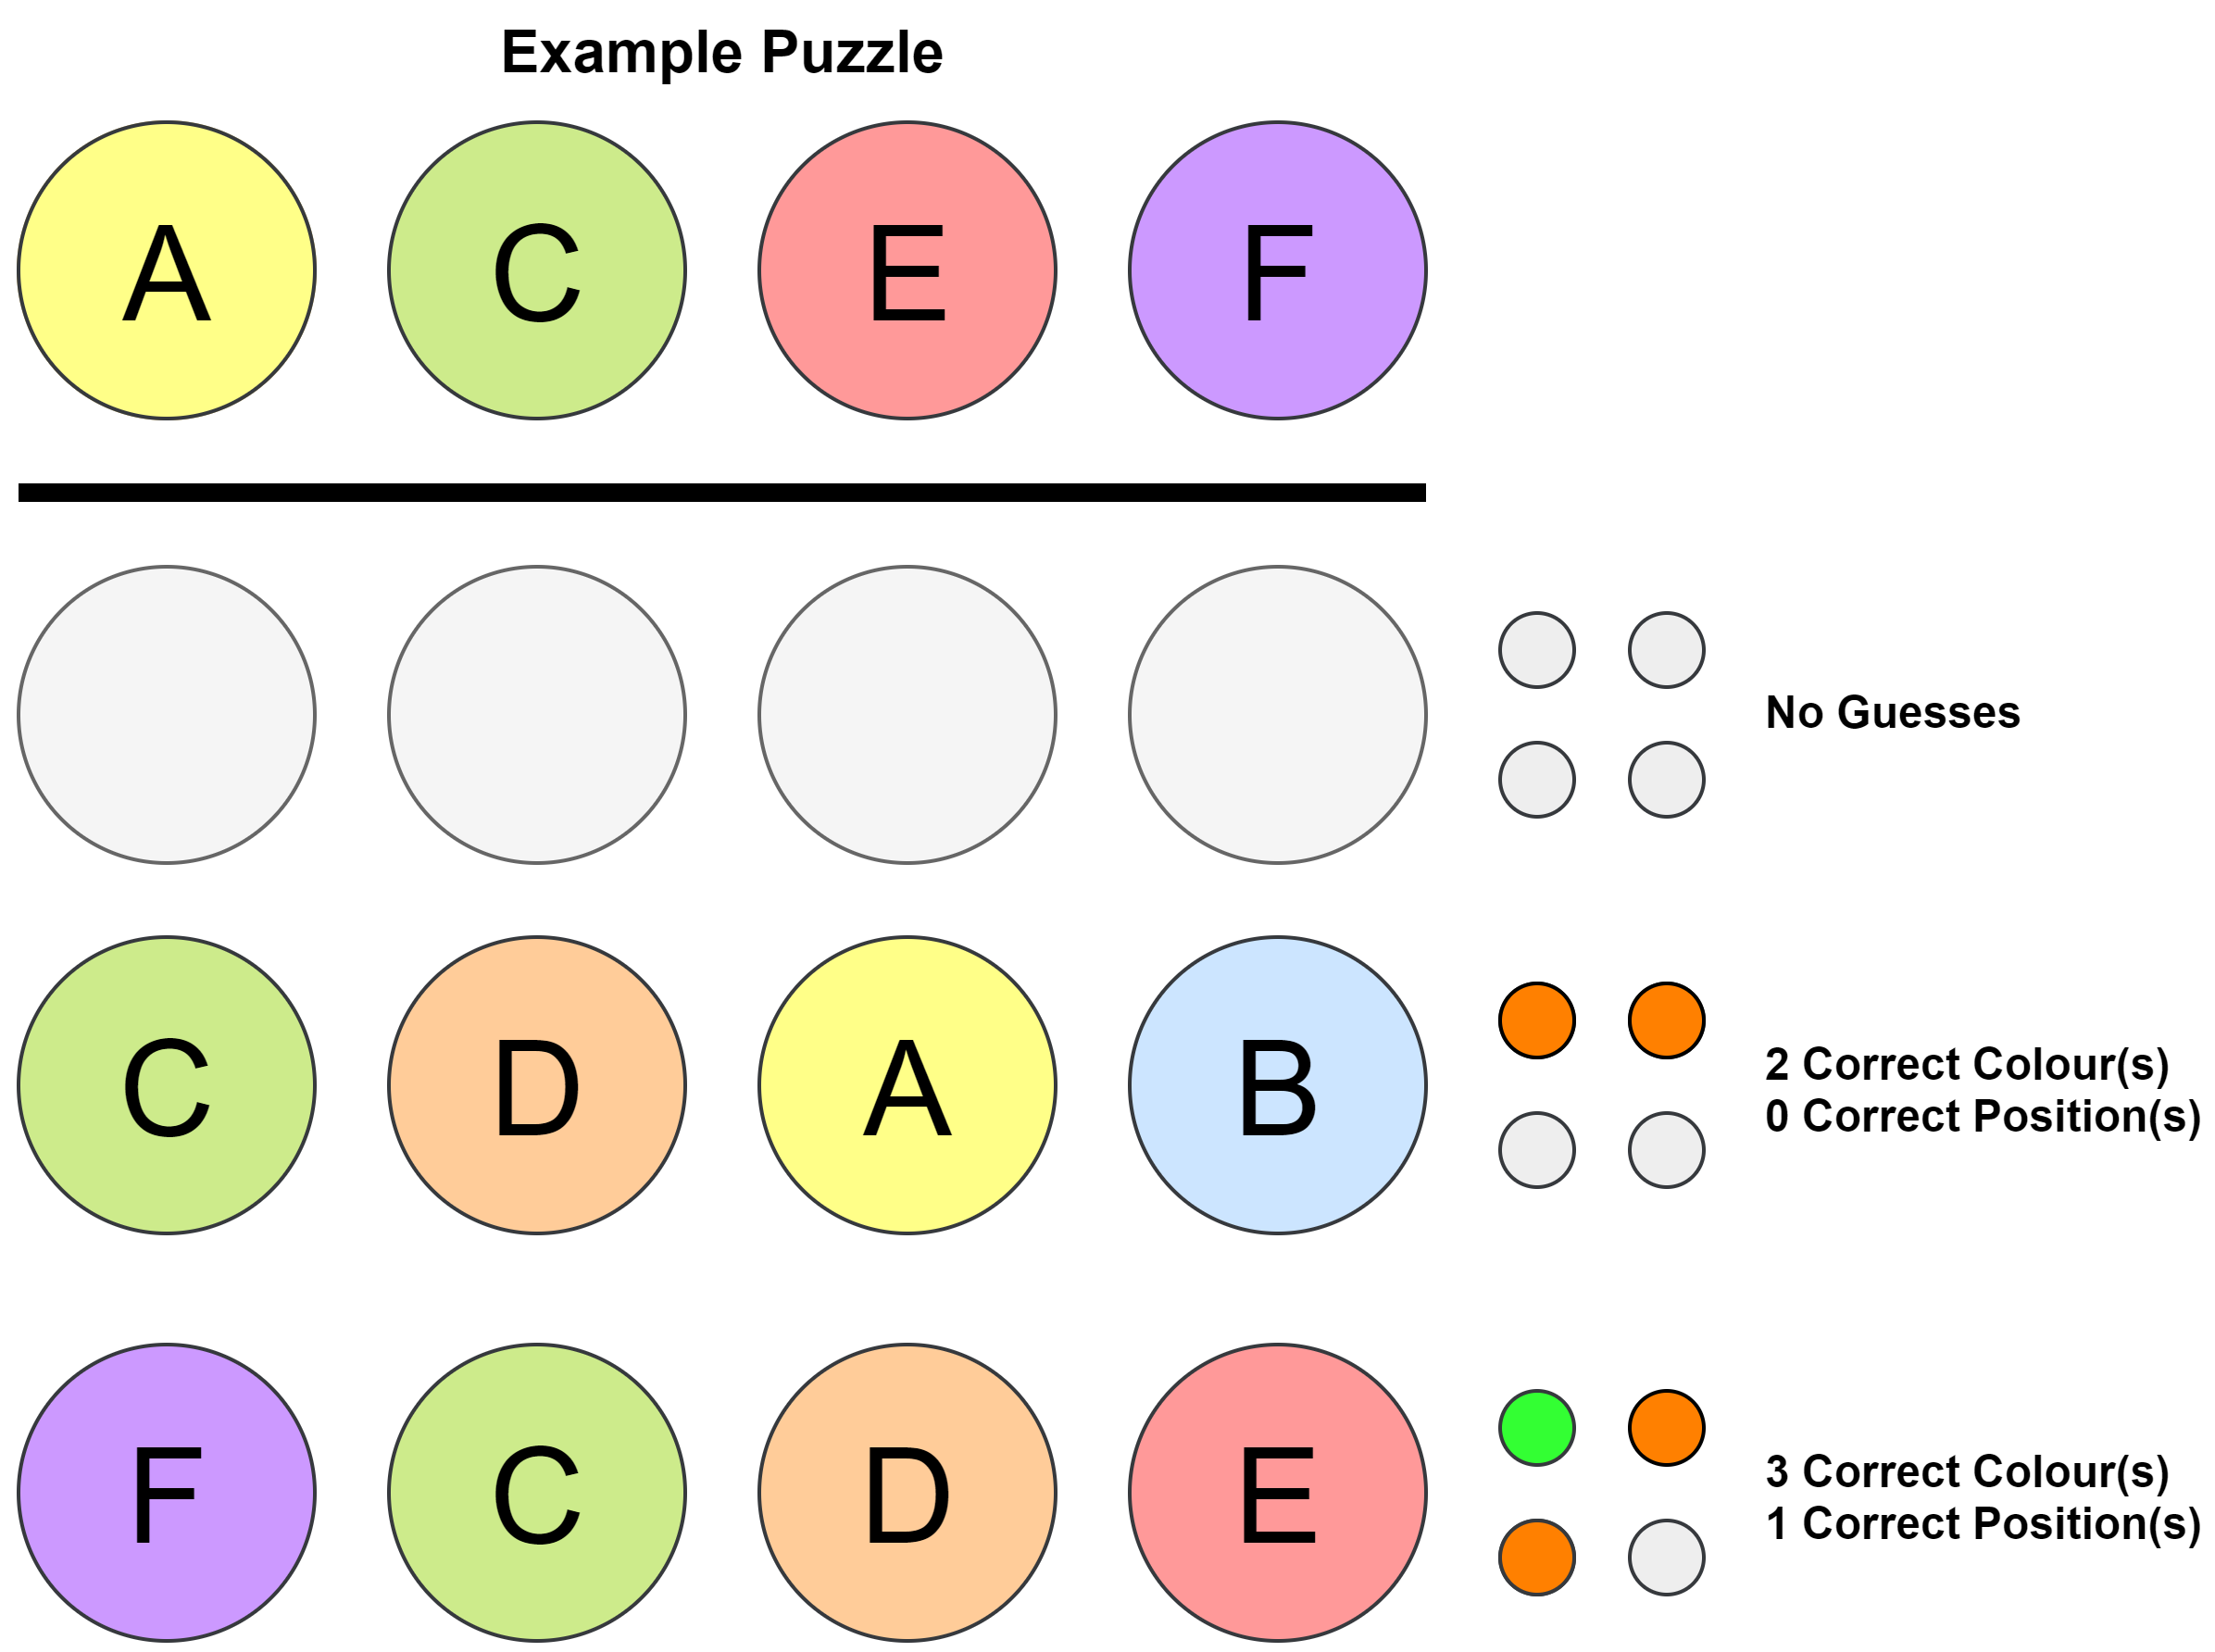
\includegraphics[scale=0.75]{guesses}
	\caption{A simplified representation of $CB$ attempting to break the code set by $CM$}
	\end{figure}
	\item {The game concludes when either the $CB$ is able to correctly guess the code set by the $CM$ or they exceed the allowed number of guesses.}
\end {itemize}

% Why is a solution to this problem important?
The game can be treated as a individual puzzle in the absence of a human $CM$ through randomly generated code combinations. This project aims to implement a solution to this puzzle that can search for the correct code combination that is comparable with exisiting solutions. The act of searching for the correct code in this context is known as a combinatorial optimization problem with a wide range of applications \cite{Haystack} and it is because of this applicability that the search for a solution is subject to continued investigation.

%%% Search Algorithms
% Which similar problems exist?

\subsection {Donald Knuth's Solution and Search Spaces}
\par One of the earliest proposed solutions to the Mastermind puzzle was a paper by Donald E. Knuth in which the claim is made that it is possible in all cases for the $CB$ to find the correct code within five attempts \cite {Wolfram} \cite {Knuth}. The solution introduces a concept which is important to solving search problems known as the \emph{consistent search space}, a term which would be defined further in later work \cite{Merelo}. The standard variant of Mastermind assumes that the code is of length four with six possible elements it can be constructed from. This definition would mean the code constructed by the $CM$ would be one of $6^4 = 1296$ possible combinations, this set of combinations is referred to as the \emph search space of the puzzle. 

\par The algorithm that Knuth proposes seeks to restrict this search space after each guess using the feedback provided by the $CM$. The algorithm proceeds after each guess by picking the best possible choice for the subsequent guess at each step, this greedy strategy \cite {Wolfram} is possible as the feedback provided can eliminate combinations which are not consistent with previously guesses. 

\par The first stage of Knuth's investigation was to define the rules of the game in a way that a computer would be able to understand. First defining the two important variables being the code $x_1 x_2 x_3 x_4$ and the test pattern, or guess, $y_1 y_2 y_3 y_4$ The initial rules that were derived were as follows:
\begin {itemize}
	\item {The number of "black hits (B)", i.e., the number of positions j such that $x_j = y_i$}
	\item {The number of "white hits (W)", i.e, the number of positions j such that $x_j =! y_j \  but \ x_j = y_k$ for some k and $y_k$ which has not at this point been a hit \cite {Knuth}.}
\end {itemize}

The process of restricting the search space can be seen in the example below with the symbols represented as integers (1, 2, 3, 4, 5, 6):
\\
{
\centering
\begin{tabular}{cccc}
No. of Guesses & Test Pattern &  Hits  & Possible Combinations \\
0 & no guess & N/A & 1296 \\
1 & 1122 &  WWW  &  16 \\
2 & 1213 &  BWW  &  4 \\
\end {tabular} \par 
} 
At the initial point where no guess had been made the search space is still comprised of all 1296 possible code combinations. This space of possible combinations is restricted using the result of the first guess which states that three of the chosen symbols were correct however their positions were incorrect. This information allows a great amount of restriction to only 16 possible code combinations which the code could belong to. The second guess restricting this space even further to just four possible combinations. Through this method Knuth asserted that it should be possible to achieve a correct guess within five test patterns. The starting pattern discovered by Knuth to give proof to this claim was found to be 1122. A possible progression of stages from this initial test pattern would be:
Another example is as follows:
\\
{
\centering
\begin{tabular}{cccc}
No. of Guesses & Test Pattern &  Hits  & Possible Combinations \\
0 & no guess & N/A & 1296 \\
1 & 1122 &  B  &  256 \\
2 & 1344 &  W  &  44 \\
1 & 3526 &  W  &  7 \\
\end {tabular} \par 
}
This situation would also allow for the next test pattern to distuingish the final possible combinations using the test pattern 1462. The algorithm places a high value on test patterns which coax the process towards the fourth guess being able to distinguish between the possible combinations. This method of solving the problem however is admitted within the paper to not be the most optimal solution. This can be shown by the way that the algorithm processes the following situation:
\\
{
\centering
\begin{tabular}{cccc}
No. of Guesses & Test Pattern &  Hits  & Possible Combinations \\
0 & no guess & N/A & 1296 \\
1 & 1122 &  BWW  &  16 \\
2 & 1213 &  BB  &  4 \\
\end {tabular} \par 
} 

which results in a possible four remaining code words (2212, 4212, 5212, 6212). The algorithm would select the test pattern 1145 as the next guess however when compared to the test pattern 4222 it can be shown that it in actuality results in less distinguishing results:
\\
{
\centering
\begin{tabular}{ccc}
Test Pattern          & Hits & Code  \\ \hline
\multirow{4}{*}{4222} & BWW  & 2212  \\
                      & BBB  & 4212  \\
                      & BB   & 5212  \\
                      & BB   & 62122 \\ \hline
\multirow{4}{*}{1145} & W    & 2212  \\
                      & WW   & 4212  \\
                      & WW   & 5212  \\
                      & W    & 62122
\end{tabular} \par
} 

It is clear that should 4222 be used at the test pattern there are two possibilities in 2212 and 4212 where the code can be known by the third guess. This is a better result compared to the test pattern 1145 where two possibilities will always be the result.

\subsection {Scoring Algorithms in Heuristics / Scoring Possible Combinations}
%%% Where is progress currently
% Donald Knuth's implementation
% Exhaustive Solutions - Most Parts, Entropy, plus & plus2

\subsection {Functional Pearls}
The inspiration for this project was a paper by Richard Bird which implemented a solution to the puzzle game Sudoku as an example of a series of problems known as functional pearls. This sections will explore the topic of functional pearls and their relevance to the current project. Functional Pearls begin as small problems which programmers wish to explore, focusing on brief but engaging examples that showcase either a guided explanation to a proof or presenation of unique data structures. The goal of a functional pearl is to teach important programming techniques and fundamental design principles \cite{Pearls}.  Richard Bird described functional pearls in a speech as 'elegant, instructive exampels of functional programming' while showcasing his implementation of a sudoku solution\cite {R. Bird Speech}.

The solution which this project aims to explore would enter the scope of a functional pearl due to its aim to document an example of functional programming. The project would however deviate from a traditional functional pearl as the scope would be expanded to consider similar solutions in the problem space to evaluate the different methods of solving Mastermind.

The functional pearl which inspired the project is Richard Birds paper 'Functional Pearl: A Program to Solve Sudoku' \cite{Sudoku}. The aim of the solution was to define the function:

\[ Sudoku :: Board \rightarrow [Board]\]

This function would take an input in the form of a Sudoku board, represented by a matrix of characters, and output a list of possible completed boards. Following this declaration the paper would proceed to use logic and equational reasoning to define the function using the functional language haskell to achieve the solution. Finally Richard Bird was able to arrive at the following definition for his solution:

\[ Sudoku :: Board \rightarrow [Board]\]
\[ Sudoku = map (map head) \bullet search \bullet prune \bullet choices\]

where search, prune and choices representing functions declared earlier in the implementation. This sudoku solutions provide an example of how the mastermind solution this project aimst to implement may be approached. Aiming for a solution that resembles this process of declaring an initial function or set of functions then deriving a defintion for them that can be evaluated through comparison with similar solutions. The next section will examine the problem that this project will aim to solve and the work that has been explored in the area previously.

\newpage                     % optional page break
\section{Research Methodology and Requirements Analysis}\label{ss:back}

The process of implementing a solution to Mastermind should consider the specifics of how the solution will be optimized. The problem space of solutions to Mastermind puzzles has been explored in multiple over investigations which necessitates that the requirements for this implementation be clearly defined and exhaustive. Guiding the declaration of how the solution should function are the set of research questions which state the purpose of the solution and what it hopes to accomplish.

\subsection {Research Methodology}
The question that this project aims to answer is 'How can the combinatorial problem of Mastermind be solved'. The scope of this question is quite large so instead it will be broken down into a set of smaller questions that will help to define the research methodology. Those questions are as such:

\begin {itemize}
	\item {How can the search space of consistent combinations be minimized}
	\item {Which scoring algorithms provide the best possible chance of selecting the correct code from a set of consistent solutions.}
\end {itemize}

\newpage                     % optional page break
\section{Evaluation Strategy}\label{ss:back}

The evaluation of the solutions implemented in this project relate strongly to the research questions that we have defined in the previous section. Following from this means that the metrics on which our solutions will be evaluated on are as such:
\begin {itemize}
	\item {A solution which is able to restrict the consistent combination search space is considered more valuable.}
	\item {A solution which is more accurate in selecting the correct code from the consistent search space is more valuable.}
	\item {A solution which is able to scale elegantly with both an increase in possible symbols which comprise the code and an increase in the length of the code.}
\end{itemize}

\newpage
\section {Preliminary Work}

In here talk about the work done with the current base solution. It will be originally done based on the donald knuth implementation.


\newpage                     % optional page break
\section{Project Management}\label{ss:back}

\subsection {File and Resource Management}

\subsection {Timeline and Deadlines}

\subsection {Risk Analysis and Mitigations}

To manage the progress of this project efficiently it was important to identify possible risks that could prevent the realisation of the goals laid out earlier in this document. To aid in the identification of the risks the following key was used to classify the associated risks:
\begin{itemize}
\item{People (P) - Risks which are the result of issues related to those individuals involved in the project. This relates to the wellbeing, scheduling and personal issues that can be encountered.}
\item{Technological (T) - Risks which can result from the technology being used to engineer the solutions. This relates to the technologial constraints that could be encountered or the hardware required.}
\item{Requirement (R)  - Risks which can result from changes to the requirements of the project. This relates to problems encountered with the work being implemented for the project. Logical problems and issues with the material involved would be included in these risks.}
\end{itemize}

\begin{tabularx}{1.1\textwidth} {
	|  >{\center\arraybackslash}X
	| >{\center\arraybackslash}X
	| >{\center\arraybackslash}X
	| >{\center\arraybackslash} X | }
	\hline
	ID & Risk & Description \\
	\hline
	P/T/R1 & Textual Title of Risk & Textual Description of the Risk \\
	\hline
\end{tabularx}

\begin{tabularx}{1.1\textwidth} {
	|  >{\center\arraybackslash}X
	| >{\center\arraybackslash}X
	| >{\center\arraybackslash}X
	| >{\center\arraybackslash} X | }
	\hline
	ID & Risk & Description \\
	\hline
	P.1 & Illness and Health Complications & The situation in which an individual involved in the project is unable to contribute due to illness or health complications. This risk is slightly heightened as the world recovers from the effects of the Covid-19 pandemic however it also considers other conditions which would require time away from the project. \\
	\hline
	T.1 & File Loss & This is the situation in which files or documents relating to the project is lost. This is a low priority issue as precautions have been taken to mitigate this such as using version control through Github. \\
	\hline
	R.1 & Insufficient Base Solution & The success of this project is dependant on having a solid base solution. The success of the base solution is assessed by a set of conditions which deems it suitable for solving the problem. The base solution being unable to meet this conditions is a serious situation and as such should be of a high priority. \\
	\hline
\end{tabularx}



%%%%%%%%%%%%%%%%%%%%%%%%%%%%%%%%%%%%%%%%%
%
%     Bibliography
%
%     Use an easy-to-remember tag for each entry - eg \bibitem{How97} for an article/book by Howie in 1997
%     To cite this publication in your text, write \cite{How97}.  To include more details such as
%     page, Chapter, Theorem numbers, use the form \cite[Theorem 6.3, page 42]{How97}.
%
\begin{thebibliography}{99}

% 
% The usual convention for mathematical bibliographies is to list alphabetically
% by first-named author (then second, third  etc. author then date)
% websites with no author names should go by the site name
%

% Typical layout for reference to a journal article
%\bibitem{Bovey}
%J. D. Bovey, M. M. Dodson,                         % author(s)
%The Hausdorff dimension of systems of linear forms % article name
%{\em Acta Arithmetica}                             % journal name - italics
%{\bf 45}                                           % volume number - bold
%(1986), 337--358.                                   % (year), page range


% Typical layout for reference to a book
%
%\bibitem{Cassels}
%J. W. S. Cassels,                                  % author(s)
%{\em An Introduction to Diophantine Approximation},% title - italics
%Cambridge University Press, Cambridge, 1965.       % Publisher, place, date.

% Typical layout for reference to a website
%
%\bibitem{GAP}
%The GAP Group, GAP -- Groups, Algorithms, and Programming,  % Site name
%Version 4.5.6; 2012. % other information
%(http://www.gap-system.org)  % URL


% Typical layout for reference to an online article

%\bibitem{Howie}
%J. Howie,                                            % author(s)
%{\em Generalised triangle groups of type $(3,5,2)$}, % article name - italics
%http://arxiv.org/abs/1102.2073                       % URL
%(2011).                                              % (year)

\bibitem {Wordle}
New York Times,
{\em "Wordle"}
https://www.nytimes.com/games/wordle/index.html
(Online, accessed 21-11-2022)

\bibitem {Wolfram}
Weisstein, Eric W.
{\em '"Mastermind." From Mathworld -- A Wolfram Web Resource'}
https://mathworld.wolfram.com/Mastermind.html
(Online; accessed 9-November-2022)

\bibitem {Invicta}
Invicta Toys and Games ltd.
{\em 'History of Mastermind'}
https://web.archive.org/web/20070812104420/http://dspace.dial.pipex.com/town/road/gbd76/toys.htm
(Archived 2007)

\bibitem {Nelson}
Nelson, Toby.
{\em 'Investigations into the Master Mind Board Game'}
https://web.archive.org/web/20150906043015/http://www.tnelson.demon.co.uk/mastermind/index.html
(1999, Archived 2015)

\bibitem {Haystack}
Merelo-Guervós, J.J., Castillo, P. and Rivas, V.M. 
{\em ‘Finding a needle in a haystack using hints and evolutionary computation: the case of evolutionary MasterMind’, Applied soft computing}
{\bf  6(2)}
(2006) pp. 170–179. 
doi:10.1016/j.asoc.2004.09.003.

\bibitem {Knuth}
Knuth, Donald E. 
{\em 'The Computer as Master Mind', Recreational Mathematics}
{\bf 9(1)}
Stanford University
(1976, Baywood Publishing Co., Inc.)

\bibitem {Merelo}
 Merelo, J.J., Mora, A.M., Cotta, C. and Runarsson, T.P. 
{\em ‘An experimental study of exhaustive solutions for the Mastermind puzzle’.}
(2012) 

\bibitem {Pearls}
Bird, Richard.
{\em How to Write a Functional Pearl}
International Conference on Functional Programming, Portland
(2006)

\bibitem {R. Bird Speech}
Gibbons, Jeremy.
{\em University of Oxford, Functional Pearls}
http://www.cs.ox.ac.uk/people/jeremy.gibbons/pearls/
(2009)

\bibitem {Sudoku}
Bird, Richard.
{\em Functional Pearl, A Program to Solve Sudoku}
Cambridge University Press, Cambridge, 2006



\end{thebibliography}
\end{document}
